
%*****************************************
\chapter{Case Study}\label{ch:fifth}
%*****************************************

In the following chapter, we will present the user case study which we conducted, to validate the findings of Anonymous et al. \cite{anonymous}, presented in Chapter \ref{ch:third}. Our goal was to verify that orientation time truly has an influence on the perceived efficiency of an authentication mechanism. In other words, given two authentication mechanisms that have the same input time, yet one has a longer orientation time than the other. Than the one with the longer orientation time is bound to be perceived as less efficient and will therefore be less favored than the other mechanism. 


\section{Design}

The user case study was designed as a field study and was conducted on campus of the computer science department of Uni Bonn and at the author's home. The independent variable was \textit{ratio} and it had three levels:
\begin{enumerate}
    \item \textcolor{blue}{Long} orientation - \textcolor{red}{Short} input, 
    \item \textcolor{red}{Short} orientation - \textcolor{blue}{Long} input,
    \item \textcolor{red}{Short} orientation - \textcolor{red}{Short} input.
\end{enumerate}

The order of the ratios was counterbalanced amongst the participants [FIGURE RATIOS]. Data was collected quantitatively by measuring the orientation and input time for each of the ratios. We also documented the number of errors made during orientation and also when a false input was made. This information was automatically documented and stored in a local database during the interaction. Data was also collected qualitatively through a questionnaire, which required study participants to evaluate the aesthetic of our application, the ratios 1) and 2), and to also choose which of the two ratios they preferred. The study was intentionally designed to be as short and simple as possible. such that we could receive the information we needed from our participants without requiring too much effort or concentration. On average the duration of the study was 15 minutes per participant. 


\section{Participants}

We were able to recruit 25 participants for our study. Initially, students were informed about the study through a Whats-app group, made for the computer science students of Uni Bonn. Another part was collected on campus of the university's computer science department, and four participants were acquaintances of the author. There was no premise for participating in the study, meaning anyone could have eligible to partake. After extracting participants that made search and inputs errors out of our sample, we remained with 19 participants, of which 13 (62.4\%) were male and 6 (31.6\%) were female. The average age was 21 years, with 17 being the youngest and 31 being the oldest. The majority of the participants (78.9\%) had an IT-Background and were computer science students. Also, all of the participants, except for one, used a screen lock for their smartphones, of which 42.1\% used PIN, 36.8\% used PATTERN, and 15.8\% used PASSWORD (see figure \ref{fig:demo}).  

%\begin{figure}[t!]
%\centering
%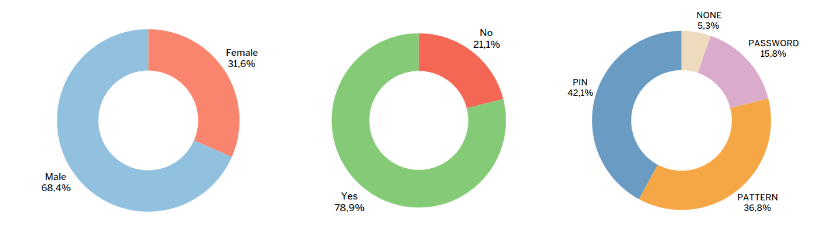
\includegraphics[width=16cm, %height=6cm]{Chapters/graphics/Demos.PNG}
%\caption{Demographic data on the gender (left), IT-Background %(middle) ration and on the personal screen lock choice (right) %of our participants.}
%\label{fig:demo}
%\end{figure}

\section{Procedure}
The study was held for each participant, separately. We began by roughly explaining the purpose of our study:

\begin{center}
\textit{To analyse certain factors in smartphone authentication that might play a role in its perceived efficiency.}    
\end{center}

We also emphasized our main focus was the improvement of usability in authentication mechanisms and that the security aspect was outside of the scope of this thesis. Also, we clarified that the testing of \underline{\textbf{FiPa}} was not intended to evaluate their skill or intelligence. We wanted our participants to feel as comfortable as possible during the course of the study and that they did not feel nervous or put under pressure. This was important to us because we wanted their performance and our collected data to be as close to the result of a real-life scenario as possible. \\

Next, we described the structure of our application, \underline{\textbf{FiPa}}. We explained that it was an interaction system which emulated an activity, similar to an authentication concept. Furthermore, we mentioned that the application presented a series of small "challenges", for them to solve. With "challenges" we meant the mental and practical tasks, explained in Chapter \ref{ch:forth}. These simple challenges were demonstrated with the help of a simple paper prototype.\\

After ensuring that our participant had no further questions, it was time for them to test \underline{\textbf{FiPa}}. First, they were asked to begin with the training-segment of the application. The purpose of the training segment was to ensure that our participant understood the concept of \underline{\textbf{FiPa}} and to prevent that our measured times be influenced by a lack of understanding of what to do. Therefore, the participant could repeat the training as often as they wanted until they felt ready to start the actual testing of the application. We guided them through the training segment, when help was needed, and took the chance to explain to them the certain features and aspects of the application. \\


When the participant felt ready to start the test, we first entered a user-id, to be able to pair their measured data with their qualitative data later, during the evaluation. We did not intervene, while they were working on the test. Once they were done, they were given a questionnaire to fill out. After the study, each participant was compensated with 5 Euros.

\section{Results}

